%*****************************************************************************************
%*********************************** Second Chapter **************************************
%*****************************************************************************************

\chapter{Methods}
\label{chap:methods}
\ifpdf
    \graphicspath{{Chapter2/Figs/Raster/}{Chapter2/Figs/PDF/}{Chapter2/Figs/}}
\else
    \graphicspath{{Chapter2/Figs/Vector/}{Chapter2/Figs/}}
\fi



\section{Petri Nets}
\subsection{Syntax and Semantics of Basic nets}
A Petri Net is a 4-tuple $(P, T, pre, post)$ defined as:
\begin{itemize}
\item[-] a set of \textit{places} (or conditions) $P$
\item[-] a set of \textit{transitions} (or events) $T$
\item[-] a \textit{preconditions map pre} : $T \rightarrow \mathbf{m}P$ which assigns a multiset of places $pre(t)$ to each transition $t \in T$
\item[-] a \textit{postconditions map post} : $T \rightarrow \mathbf{m}P$ which assigns a multiset of places $post(t)$ to each transition $t \in T$
\end{itemize}
where $\mathbf{m}P$ is the space of multisets over $P$ with a multiset
over P defined as function $f: P \rightarrow \mathbb{N}$. The state of
the system, called a marking, is again a multiset $\mathcal{M}$ over
$P$. We can think of the marking as the distributed global state of
the system. It is also common when defining a Petri Net to give the initial marking of the system usually written as $\mathcal{M}_0$.

Markings can change as transitions occur:
\begin{equation*}
\mathcal{M}\overset{t}{\longrightarrow}\mathcal{M^\prime}
\end{equation*}
The change in the marking through the action of transition $t$ is
defined in the $pre$ and $post$ maps:
\begin{equation*}
\mathcal{M}\overset{t}{\longrightarrow}\mathcal{M^\prime} \mbox{ iff } pre(t) \leq \mathcal{M} \mbox{ and } \mathcal{M^\prime} = \mathcal{M} - pre(t) + post(t)
\end{equation*}
There is a widely used graphical notation for Petri Nets where
transitions are represented by squares, places by circles, and the
condition maps with directed weighted edges between the two types of
nodes(squares and circles). Edges defined in the $pre$ map are
represented as inbound edges and edges defined in the $post$ map are
defined as outbound edges. Markings are represented by tokens inside
the place. For example a Petri Net with three places and the following
marking,
\begin{equation*}
M_{p1} = 2\mbox{, } M_{p_2}=1 \mbox{ and } M_{p_3} = 2
\end{equation*}
, would be represented by 2 tokens residing in the circle for place
$p_1$, 1 token in the circle for place $p_2$, and 2 tokens in the
circle for place $p_3$. If the net also has one transition $t_1$ and
the following maps,
\begin{equation*}
pre(t_1) = (p_1 = 2, p_2 = 1, p_3=0) \mbox{ and } post(t_1) = (p_1
=0, p_2=0, p_3=2)
\end{equation*}
then the net would have inbound edges from $p_1$ and $p_2$ to the
transition node weighted with 2 and 1 respectively and an outbound edge
weighted by 2 between the transition node and the circle representing
$p_3$(Figure~\ref{fig:pn_example}). The places connected with
inbound edges with a transition are called the pre-places and the
places connected with outbound edges with a transition are called the
post-places of that transition. When a transition fires, tokens are removed from its
pre-places and are placed in its post-places according to the weights
on the corresponding edges. For example in the previously defined net,
if transition $t_1$ fires 2 tokens will be removed from $p_1$, 1 token
from $p_2$, and 2 tokens will be added to place $p_3$(Figure~\ref{fig:pn_operation}).

\begin{figure}
\centering
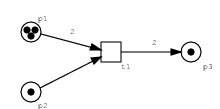
\includegraphics[scale=1.0]{pn_example}
\caption{Small basic Petri Net example}
\label{fig:pn_example}
\end{figure}

\begin{figure}
\centering
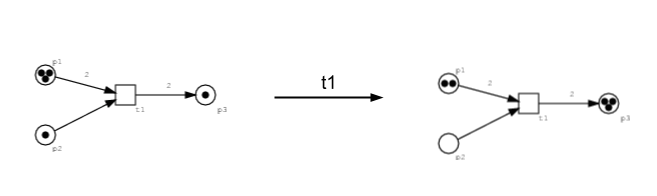
\includegraphics[scale=0.7]{pn_operation}
\caption{The token game for basic Petri Nets.}
\label{fig:pn_operation}
\end{figure}

This graphical view of the operational semantics of Petri Nets is
usually referred to as the 'token game' because of this flow of tokens
from pre-places to post-places for every transition that occurs. This
leads to a simple algorithm for the execution of Petri Net models:

\begin{enumerate}[noitemsep]
\item Initialise the net  with $(P, T, pre, post)$ and set state $\mathcal{M} = \mathcal{M}_0$
\item Find enabled transitions, $enabled \subseteq T, \forall t \in T \mbox{ if } pre(t) \leq M$
\item Choose transition $t$ from set of enabled at random
\item Update state according to $\mathcal{M} = \mathcal{M} -pre(t) + post(t)$
\item Repeat steps 2-4 until there are no more enabled transitions or an external stop condition is met(e.g. max number of steps)
\end{enumerate}
Non-determinism comes in the system from step 2 where we choose a
transition to fire at random from a set of enabled ones. This way multi-option
probabilistic decisions can be incorporated by having one or more
transitions that share pre-places. From the
example Figure~\ref{fig:nondet} when the shared pre-place is
sufficiently marked both transitions would be enabled. The token would
have to make a non-deterministic decision between the two
alternatives, $t_1$ and $t_2$, and flow to the corresponding
post-place.

\begin{figure}
\centering
\includegraphics[scale=0.7]{nondet}
\caption{Non-deterministic decisions encoded in Petri Net structure.}
\label{fig:nondet}
\end{figure}

There is a very natural correspondence Petri Nets and biochemical
systems. Every reaction is represented by a transition with the
reactants becoming pre-places and the products post-places of that
transition. The stoichiometry of a reaction is represented in the
pre and post maps. A reaction like $2H + O \rightarrow H_2O$ will lead
to a Petri Net with three places and one transition removing two
tokens from the $H$ places and 1 token from the $O$ place and adding
one token to the $H_2O$ place. The tokens in each place indicate the
amount of the corresponding species. Notice that despite the
fact that there is an implicit ordering of events during the execution
of the net, time is not explicitly modelled. Hence biological models
captured with simple Petri Nets cannot capture the dynamic behaviour
of the system. They have however been used for qualitative modelling
of metabolic pathways using their structural and
marking-dependent properties. The fact that they do not model time has
another implication in that all reactions are equally likely to
happen when they are enabled. In decision structures, like the one in
Figure~\ref{fig:nondet}, all the available options are equally
likely. This decision process is crucial in our use-case therefore we
need more tight control, for example being able to set the
probabilities of the outcomes. This makes basic Petri Net an unsuited
language for our purposes so we used an extension, Stochastic Petri
Nets, that is described in the next section.

\subsection{Stochastic Petri Net extension}
Stochastic Petri Nets explicitly model time by introducing a wait time
for each transition. Wait times are random variables that follow an
exponential distribution with the rate of the transition. Stochastic
Petri Nets are a 5-tuple $(P, T, pre, post, \nu)$. Everything is
defined as before with the only addition being the $\nu$ that is a
map between transitions and rate functions. A rate function for a
transition $t$ is a
possibly marking dependent function that returns the rate
$\lambda(M)_t$ for the wait time of that transition. Now the
operational semantics also change slightly. When a transition $t$ is
enabled a wait time is sampled from a negative exponential with rate
$\lambda(M)_t$ which has to lapse before the transition
fires. Therefore time is explicitly captured. When more than one
transition is enabled a wait time is sampled from all of them and the
one with the least wait time gets to fire. This suits our modelling
requirements for assigning probabilities to outcomes of
non-deterministic decisions. For a decision structure like the one in
Figure~\ref{fig:nondet} we can set the likelihoods of the two outcomes
$t_1$ and $t_2$ by adjusting their relative rates $\lambda_{t_1}$ and
$\lambda_{t_2}$. 

\section{Stochastic Pi-calculus}
Pi-calculus is a process algebra designed to capture decentralised
computation as the action of independent agents/processes which
communicate with each other. Stochastic pi-calculus is an extension to
the original formulation to capture stochasticity and time similar to
the Stochastic Petri net extension for basic Petri Nets. Processes can
do a sequence of actions which are composed with the '.'(dot)
operator. Each action can be a receive or send 
action. Communication between processes is done with
message-passing through send/receive actions between procesess. For
example consider a process A:
\begin{equation*}
A = !a.?b.P
\end{equation*}
The behaviour of $A$ is a chain of events composed with the
\texttt{.} operator. First $A$ offers to send a message on channel
\texttt{a}, then it offers to receive a message on channel \texttt{b}
and then it evolves into a process P. Communication happens between two
processes that offer to receive and send on the same channel. Consider
the following evolution of a system consising of two parallel processes(composed
with the '|' operator):
\begin{equation*}
(!a.?b.P) | (?a.Q) \Rightarrow (?b.P) | Q
\end{equation*}
Once the communication via channel \texttt{a} happens, both processes
move to the next action in their sequence. Communication over a
channel has the ability to pass messages between the two processes
that can be further used in subsequent actions. This message passing
feature is mainly used to pass private channels, which can be created
by processes, for private communication.Non-determinism is added to
the system by having a choice operator '+'. This operator can join
sequence of actions together. For example consider an extension to the
$A$ process we defined above:
\begin{equation*}
A = !a.?b.P + ?c.Q
\end{equation*}
Now A has a choice between two series of actions. If the first action
for both series can occur then one of them is chosen
non-deterministically. This is equivalent to the decision structure we
have seen in the basic Petri Nets. As was the case with the Stochastic
Petri Net extension, Stochastic pi-calculus adds a wait time or
communication delay for every channel which is distributed
exponentially with a rate specific to that channel. If more than one
communication action can happen the one with the least delay in its
channel will occur. This mechanism again allows us to encode
probabilities of options for decisions.

In this study we used SPiM which is a programming language based on
stochastic pi-calculus with a well-degined syntax that
one can use to program a biological model. It also, and more
importantly, has a graphical notation which corresponds to the textual
notation. The language operators change slightly and the language is
more like a traditional programming language. To see the
correspondence, two parallel process in pi-calculus, $ (!a.?b.P + ?c.Q) |
(?a.Q)$, become the following SPiM program:
\begin{verbatim}
new a@0.3: chan
new b@0.5: chan
new c@0.4: chan

let A()=
(
    do !a; ?b; P()
    or ?c; Q()
)
and P()=()
and Q()=()
and B() = ?a;Q()

run (A()|B())
\end{verbatim}
Channels can be declared with the \texttt{new} keyword and processes
similar to how functions are traditionally declared in programming
languages. Processes can also take arguments which is one difference
between SPiM and traditional stochastic pi-calculus. The '+' operator for choice becomes a 'do or' statement,
the dot operator becomes ';'. Another addition to the notation is the
'delay' operator which can be used to delay an action with an
exponentially distributed wait time based on the rate of that delay:
\begin{verbatim}
let A = delay@0.3;!a;()
\end{verbatim}


The graphical notation for the above
system is given in Figure~\ref{fig:sp_graph}. We can think of this
notation as representing state transitions again but this time between
different states of one components/process. This notation emphasises
the fact that the behaviour of each component is defined
independently. A node stands for a process state and there is an edge
between two nodes labelled with an action if it is possible to go from
one process state to the other through that action. A new state of a
process could a new process. Choice is represented by having two or
more outgoing edges from a process state.

\begin{figure}
\centering
\includegraphics[scale=0.3]{sp_graph}
\caption{Graphical notation for SPiM}
\label{fig:sp_graph}
\end{figure}

The processes and communications of pi-calculus are very generic and
can be used for all systems of interacting agents that communicate. In
biochemical systems molecules become processes and their communications
are the reactions. Defining a pi-calculus model is not a straight
translation from a series of reactions because reactions are broken
down to a send and receive part which are then defined as actions for
the reactant proesses. The products of the reaction are defined as the
reactant processes evolving to a new process after the
communication. Despite the fact that the model is not defined in
terms of reactions but in terms of species, the evolution of a
pi-calculus model is still reaction-centric since the basic unit of
computation is a communication event between two processes. Also
the decision between reactions can be encoded nicely with the choice
operator. These characteristics meet our requirements for a language
to capture a reaction-centric view of the system. Their different
approach in system definition along with their graphical notation
makes for an interesting alternative to Petri Nets which are closer to
the standard chemistry view of the system as series of reactions.